\documentclass[tikz,border=2pt]{standalone}
\usepackage{amsmath,amssymb}
\usepackage{pgfplots}
\pgfplotsset{compat=1.18}

\begin{document}
% Chernoff bound for X ~ Exp(1), a = 3: every t in (0,1) gives the bound e^{-3t}/(1-t); the best
% one is at t = 2/3 (3e^{-2} = 0.406). The exact tail is e^{-3} = 0.050.
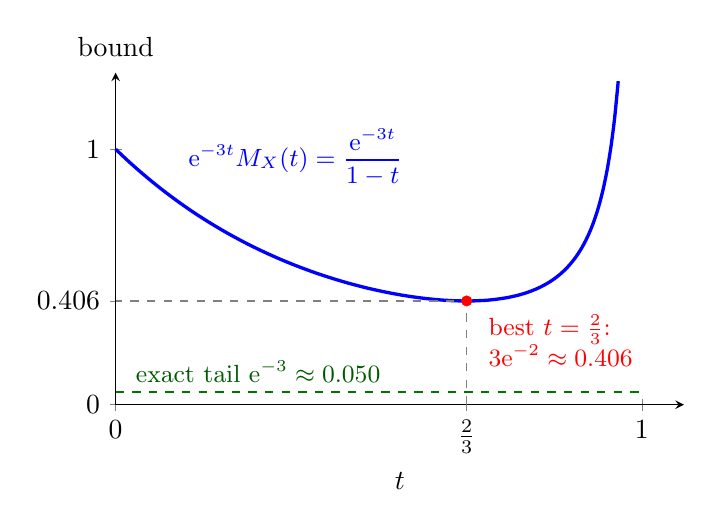
\begin{tikzpicture}
	\begin{axis}[
		axis lines=left, xmin=0, xmax=1.08, ymin=0, ymax=1.3,
		xtick={0,0.667,1}, xticklabels={$0$,$\tfrac23$,$1$}, ytick={0,0.406,1}, yticklabels={$0$,$0.406$,$1$},
		xlabel={$t$}, ylabel={bound}, ylabel style={rotate=-90, anchor=south, at={(axis description cs:0,1.02)}},
		samples=140, smooth, width=8.8cm, height=5.8cm, clip=false
		]
		\addplot[blue, very thick, domain=0:0.955] {exp(-3*x)/(1-x)};
		\draw[gray, dashed] (axis cs:0.667,0) -- (axis cs:0.667,0.406) -- (axis cs:0,0.406);
		\fill[red] (axis cs:0.667,0.406) circle (2pt);
		\node[red, anchor=north west, font=\small, align=left] at (axis cs:0.69,0.39) {best $t=\tfrac23$:\\ $3\mathrm{e}^{-2}\approx0.406$};
		\draw[green!45!black, thick, dashed] (axis cs:0,0.0498) -- (axis cs:1.0,0.0498);
		\node[green!35!black, anchor=south west, font=\small] at (axis cs:0.02,0.05) {exact tail $\mathrm{e}^{-3}\approx0.050$};
		\node[blue, anchor=south west, font=\small] at (axis cs:0.12,0.82) {$\mathrm{e}^{-3t}M_X(t)=\dfrac{\mathrm{e}^{-3t}}{1-t}$};
	\end{axis}
	
\end{tikzpicture}
\end{document}
